\subsection{Background}
% Mathematical and historical background and major applications, including references
\textcolor{blue}{To be written by Hossein}

\subsection{Code structure and functionalities}
% Where classes are located and what abstract classes represent
\textcolor{blue}{To be written by Hossein}

\subsubsection{Fourier transform algorithms}
% Description of each algorithm, with the iterative one in detail, mentioning OpenMP
\textcolor{blue}{To be written by Hossein}

\subsubsection{Bit reversal permutation algorithms}
We implemented three different bit reversal permutation algorithms. The class \texttt{Naive\-Bit\-Reversal\-Permutation\-Algorithm} contains a naive implementation, used for testing for correctness. The class \texttt{Mask\-Bit\-Reversal\-Permutation\-Algorithm} was adapted from \cite{mask_bit_rev} and follows a similar approach, but it is made more efficient using biwise operators, bit masks and bit shifts. Both these implementations have a time complexity of $O(n log(n))$, but the latter has a very small constant. Moreover, both implementations loop over the entire sequence and calculate the bit reversed representation of each index. As such, this loop is easily parallelizable. The third implementation can be found in \texttt{Fast\-Bit\-Reversal\-Permutation\-Algorithm}, it was adapted from \cite{fast_bit_rev} and has a time complexity of $O(n)$. While asymptotically better performing than \texttt{Mask\-Bit\-Reversal\-Permutation\-Algorithm}, this implementation performs worse for small sequences and has worse parallel scaling. 

All implementations were parallelized using OpenMP. Moreover, the implementation in \texttt{Mask\-Bit\-Reversal\-Permutation\-Algorithm} calls the function \texttt{Mask\-Bit\-Reverse} in a loop, which was declared using the pragma \texttt{\#pragma omp declare simd} with some additional clauses, to allow the compiler to more easily perform vectorization.

\subsection{Results}
We performed performance and parallel scaling tests using a consumer-grade device, with an AMD Ryzen 9 5900HX CPU with 8 physical cores, 16GB of DDR4 RAM and using WSL as an operating system. Results for the implementation in \texttt{Iterative\-Fourier\-Transform\-Algorithm} use an instance of \texttt{Mask\-Bit\-Reversal\-Permutation\-Algorithm} for the bit reversal permutation step and are relative to the direct transform. Unless otherwise stated, all sequences used for testing are randomly generated sequences of complex numbers, using doubles to represent each of the real and immaginary field, using \texttt{std::complex}. 

Using a sequence with $2^{19}$ elements and calculating the minimum execution times over 100 runs, the iterative algorithm with 8 OpenMP threads was $26.55x$ faster than the recursive one and $1.73x$ faster than the one implemented in the library Numpy. While the latter result is likely partially due to the small overhead for using Numpy functions and methods, this shows that our implementation is more than capable of competing with it for sequences of this size. Moreover, with the same number of runs but a sequence of just $2^{12}$ elements, the iterative algorithm is $969.32x$ faster than the $O(n^2)$ implementation. This shows how the introduction of FFT algorithms makes executing the Fourier Transform of a sequence of $2^{19}$ elements computationally simple even on a consumer-grade device, whereas executing the same transform with the $O(n^2)$ implementation would have taken about 18 hours on the same hardware. These results were obtained using the script \texttt{compare-methods.py}.

Moreover, we performed scaling tests with respect to both the number of OpenMP threads and the length of the sequence, using the scripts \texttt{compute\--performance.py} and \texttt{compute\--scaling.py} respectively. In Figure \ref{fig:fft_threads} the average execution time over 1000 runs for a sequence of $2^{19}$ elements can be seen for 1, 2, 4 and 8 OpenMP threads. In Figures \ref{fig:fft_floats} and \ref{fig:fft_doubles} the speed-up trend for multiple sequence lengths for floats and doubles respectively can be seen. Results refer to minimum execution times over 1000 runs.

\begin{figure}[ht]
    \centering
    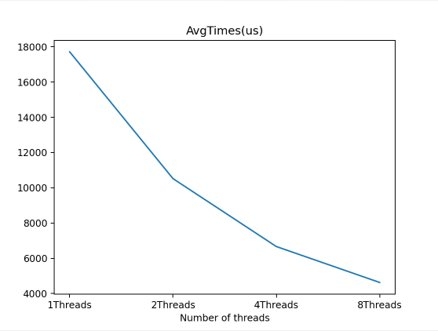
\includegraphics[width=70mm]{image/fft_times}
    \caption{Parallel scaling test with $2^{19}$ elements.}
    \label{fig:fft_threads}
\end{figure}

\begin{figure}[ht]
    \centering
    \subfigure[Speed-ups for floats]{\label{fig:fft_floats}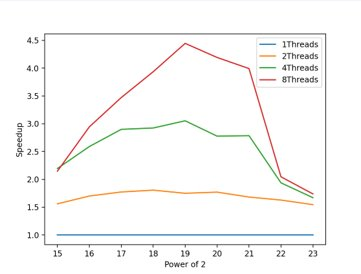
\includegraphics[width=55mm]{image/fft_scaling_floats}}
    \subfigure[Speed-ups for doubles]{\label{fig:fft_doubles}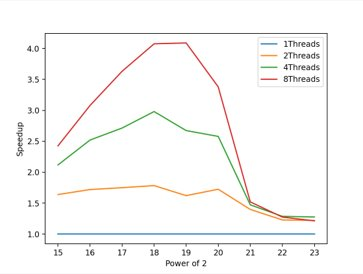
\includegraphics[width=55mm]{image/fft_scaling_doubles}}
    \caption{Scaling test with respect to the sequence length.}
    \label{fig:fft_performance}
\end{figure}

Figures \ref{fig:fft_floats} and \ref{fig:fft_doubles} show the expected trend of increasing speed-up up to a certain number of threads, as the overhead for OpenMP communication is hidden by the larger sequence sizes. However, when reaching $2^{22}$ and $2^{21}$ elements for floats and doubles respectively, the speed-up decreases drastically. We believe this behaviour is related to the size of the L3 cache of the machine, as $2^{21}$ double complex values and $2^{22}$ float complex values both require 32 MB of memory, while the L3 cache of the machine is 16 MB large. We believe that the processor is unable to perform caching effectively due to the complex access pattern to memory, causing a large number of cache misses. Therefore, while for smaller sequences the entire sequence can fit in the L3 cache, for these values part of the sequence has to be read and written from the global memory at each iteration, causing a major bottleneck for execution time. This hypotesis is supported by tests performed on another machine. Said machine's L3 cache is 4 times smaller and a similar trend can be seen, but for sequences that are 4 times smaller.